\section{Detection \& Eviction}
\label{sec:detection}

In this section, we describe the main building blocks that constitutes proposed detection mechanism that targets detecting malicious peers in order to restore benign peers satisfaction.
We start by highlighting the general overview on how the detection mechanism flows.
Then, we describe the main differences between detecting a dropping attack behavior and detecting a manipulation/outdated chunks attack behavior, referred to as \textit{drop} attack, \textit{manp} attack for simplicity.
Afterwards, each detection sub-block, as illustrated in Figure~\ref{detection-blocks}, is presented.
The list of variables used throughout the paper is provided in Table \ref{tab:acronyms}.

\begin{table}[ht]
\center
\caption{Acronyms}
\begin{tabular}{|c|l||c|l|}
\hline

\bf{Var.} & \bf{Description}  & \bf{Var.} & \bf{Description} \\\hline\hline
$x$ & no. of malicious peers & $\eta$ & mal. headnodes fraction\\\hline
$MN$ & malicious neighbors & $\sigma$ & satisfaction threshold\\\hline
$H_n$ & list of headnodes & $P_n$ & potential candidates list \\\hline
$\alpha$ & manipulation threshold& $F$ & familiarity of suspect \\\hline
$G$ & suspect guilt value & $\kappa$ & dropping det. allowed\\\hline
$NL$ & neighbor list & $BM$ & buffer map\\\hline
\end{tabular}
\label{tab:acronyms}
\end{table}

\subsection{Mechanism Overview}
Here we describe an overall view for the flow of the detection mechanism before every process is detailed through the rest of the section.
Once a detection condition is triggered by a peer $b$, it sends a detection request to all peers that exist in its neighbor list.
Afterwards, each peer who receives a request, prepares a reply according to whether the it is a \textit{drop} or a \textit{manp} request.
Once $b$ collects all the replies, it decides according to aggregated data in the replies, whether to fire a complaint, on behalf of the participating peers who also suspect $m$, to the source or not.
Finally, if $b$ sends a complaint to the source, the source decides about its content and replies back to $b$. In turn, $b$ forwards the source reply to the other participants in the complaint.

\subsection{Drop vs. Manp Detection}
According to the 
On one hand, when $m$ conducts a drop attack on $b$, $b$ is not capable of detecting any malicious behavior.
Specifically, in a drop attack, $m$ never sends the actual $BM$ that represents the chunks it currently acquires.
Hence, $m$ appears as unsatisfied benign peer to $b$.
In turn, while $b$ is still unsatisfied, it can not detect a certain suspect. 

On the other hand, in a manipulation or outdated chunks, $m$ indeed is eventually suspected to be malicious as $b$ already expects the requested chunk to be sent from $m$ as $m$ claimed.
Thus, eventually $b$ can suspect $m$ as being malicious.
To that end, through the rest of the section, we describe how the detection mechanism handles the aforementioned cases separately.

\begin{figure}
 \centering
 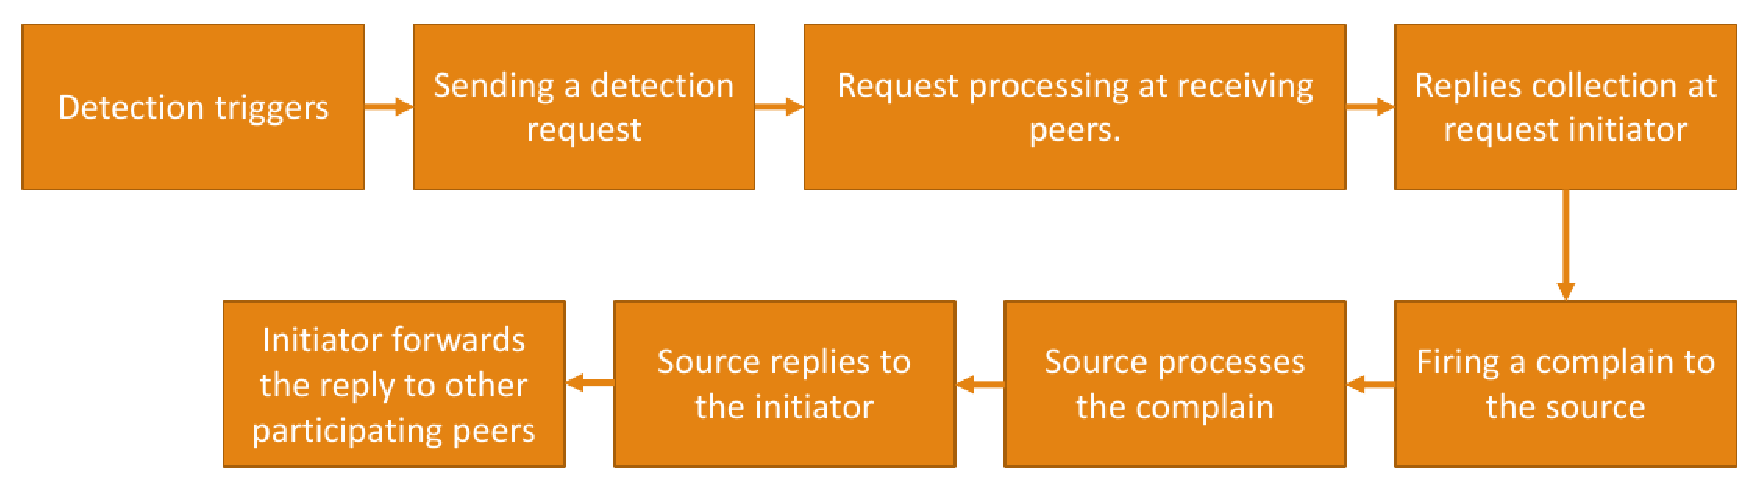
\includegraphics[width=8cm,height=3cm]{./Figures/detection-blocks.eps}
  \caption{Detection mechanism main blocks}
\label{detection-blocks} 
\end{figure}

\subsection{Detection Trigger}
Here we describe how a peer decides on sending a detection request for both attack behaviors.
In both cases, once $b$ decides on sending a detection request, it only send it to peers in its own neighbor list $NL$ to check if those neighbors agree with it or not, disregarding the source if $b$ is a headnode.

Afterwards, as detailed in Section~\ref{Firing_a_Complain}, once $b$ receives its neighbors replies to the detection request, $b$ decides whether or not to fire a complaint to the source.
We assume that the source's address is publicly known and any peer can send a complaint to the source directly whether the source is already a neighbor to this peer or not.
\subsubsection*{Drop trigger}
In this, as there is no evidence of a manipulation from any neighbor to $b$, the only factor that $b$ is concerned about is the satisfaction threshold $\sigma$.
The satisfaction of a peer is defined as the fraction of missed chunks, i.e., the continuity of the stream according to the $Hit/Hit+miss$ chunk ratio.
In details, $b$ decides to trigger a detection request only if:
\begin{enumerate}
 \item $b$'s instant $satisfaction level < \sigma$.
 \item Number of drop detections sent by $b$ in the last $1000s$ is $< \kappa$.
\end{enumerate}
The latter condition guarantees that any peer can not trigger multiple detection requests in parallel so that: (a) to avoid exhausting the source's bandwidth, and (b) the source is most likely processing another peer's dropping request that might eventually positively impact $b$'s satisfaction level.
Note that in a drop attack, the detection request sent to $b$'s neighbors does not contain a certain suspect, hence, peers receiving a suspect-less request are aware that indeed it is a drop attack request.

\subsubsection*{Manp trigger}
$b$ decides to send a detection request if it was manipulated $\alpha$ times by $m$.
This condition essentially guarantees that any peer is not suspected instantly if it did not deliver the requested chunk, i.e., a benign peer might not deliver a chunk to the requester if it is already loaded serving other peers.
Obviously, $b$ attaches the suspect ID in the detection request to its neighbors.

In order to avoid malicious peers from abusing the manipulation detection mechanism, $b$ informs $m$ when $\alpha_m = \alpha -1$.
Accordingly, $m$ should give highest priority to $b$ and send the requested chunk signed and waits for a signed Ack from $b$ as an evidence for not manipulating.
This evidence is later needed for the source to decide about $m$, as discussed in Section~\ref{Firing_a_Complain}.

\subsection{Processing Detection Request}
Here we describe how a peer $s \in S_b$, where $S_b$ is the set of peers who received a detection request from $b$ prepares a detection reply.
Note that as malicious peers the replies differ according to whether $s$ is malicious or benign, thus, we distinguish those two cases below. We refer to a malicious recipient as $s_m$ and a benign one as $s_b$.

\subsubsection*{Benign recipient}
Once $s_b$ receives a \textit{drop} request, it replies with its current satisfaction level as there is no exact suspect to give a detailed opinion about.
In case the request is a \textit{manp}, $s_b$ generates a reply the following three factors:
\begin{enumerate}
 \item \textit{familiarity $F$}: if $s_b$ is familiar with the suspect or not, i.e., is the suspect a current or a former neighbor of $s_b$ or not.
 \item \textit{Guilt $G$}: number of manipulation evidences $s_b$ has against the suspect. Note that this number is always $<\alpha$, otherwise, $s_b$ triggers a detection request on its own.
 \item \textit{Satisfaction}: the current satisfaction level of $s_b$.
\end{enumerate}


\subsubsection*{Malicious recipient}
Clearly, a malicious peer always colludes with the other malicious peers in the overlay. Hence, $s_m$ should always try to convince the detection initiator $b$ that it is fully satisfied in a \textit{drop} request.
In a \textit{manp} request, $s_b$ replies with $F=true, G=0, satisfaction=1$ in case the suspect is a malicious, as those values guarantees to convince $b$ that $s_m$ does not agree with firing a complaint to the source, as detailed in Section~\ref{Firing_a_Complain}.

\subsection{Firing a Complain}
\label{sec:Firing_a_Complain}

\subsection{Processing a Complain at the Source}
\label{sec:complaint_source}

\subsection{Processing a Complain Reply \& Forwarding}







